% ---------------------------------------------------------------- Method validation: setup
\section*{Method validation}

\subsection*{Workloads and recorded runs}
We recorded \nRuns{} complete training runs on four workloads (Table~\ref{tab:workloads}). Each workload is a grid of six learning rates, two batch sizes (64, 256) and three seeds (0, 1, 2), trained for $T=\X{budget}$ epochs on a fixed 4{,}000-image subset of the official training split, with validation loss and accuracy measured after every epoch on 2{,}000 images of the official test split. The CNN workloads use Adam~\cite{kingma2015adam}; the MLP workload uses SGD with momentum 0.9~\cite{sutskever2013momentum}, so that the gate also meets an optimiser whose curves look different. The learning-rate grids span stable, fast and unstable training: some runs are still improving at epoch 40, others overfit within a few epochs, and some diverge or stall (Fig.~\ref{fig:curves}). All runs use the same PyTorch~\cite{paszke2019pytorch} training script that the controller launches in deployment, with in-process data loading and two CPU threads per run. Re-running a configuration with the same seed reproduces its recorded curve exactly; we checked this for the first two epochs of the first Fashion-MNIST run, whose losses matched the stored values bit for bit.

\begin{table}[t]
\centering
\caption{The four workloads. Each has 36 uncontrolled runs (6 learning rates $\times$ 2 batch sizes $\times$ 3 seeds, 40 epochs). Accuracy is the median over runs of the best validation accuracy; ``best epoch'' is the median epoch of minimum validation loss; ``late'' is the share of runs whose minimum falls in the last five epochs; time is the mean wall-clock time per epoch on two CPU threads.}
\label{tab:workloads}
\footnotesize
\setlength{\tabcolsep}{4pt}
\begin{tabular}{llllrrrr}
\toprule
Dataset & Model & Optimiser & Learning rates & Acc.\ (\%) & Best ep. & Late (\%) & s/ep. \\
\midrule
\tabinput{generated/table_workloads.tex}
\bottomrule
\end{tabular}
\end{table}

\begin{figure}[t]
\centering
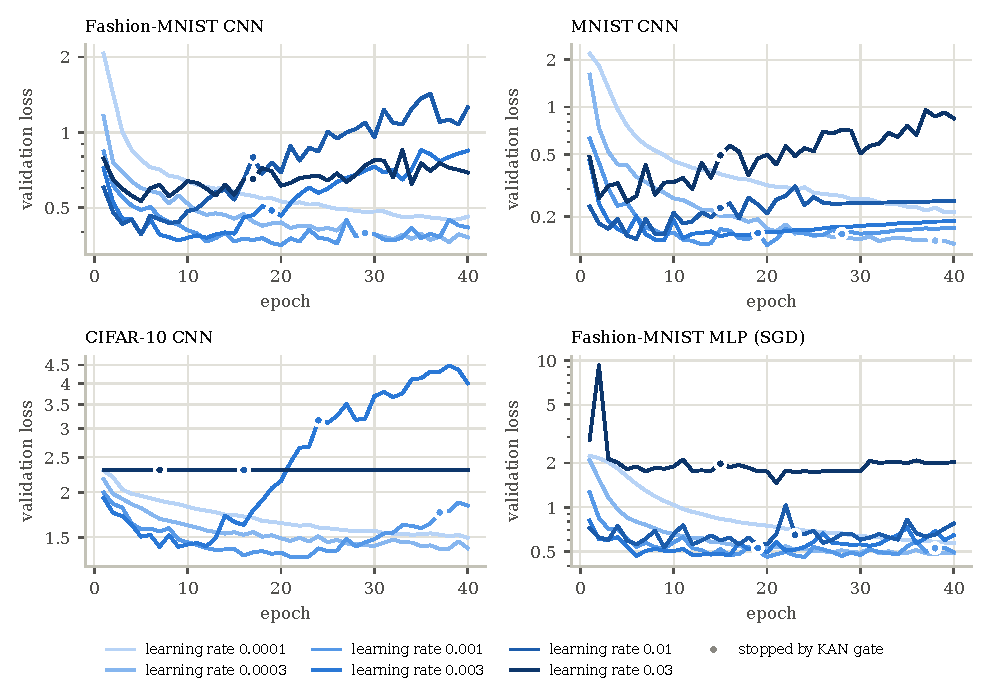
\includegraphics[width=\textwidth]{figures/curves.pdf}
\caption{Validation loss of the six learning rates (batch size 64, seed 2) on each workload, log scale. Dots mark where the KAN gate trained on the \emph{other three} workloads stops each run (leave-one-workload-out, mean over three gate seeds); runs without a dot were trained to the full budget.}
\label{fig:curves}
\end{figure}

\subsection*{Evaluation protocol}
\paragraph{Counterfactual replay} Every stopping policy is replayed on the recorded curves: at each decision epoch $t\in\{4,6,\dots,38\}$ the policy sees the run's history up to $t$ and either continues or stops. A policy that stops at epoch $t$ is credited with the best validation loss observed up to $t$, which is what a practitioner who checkpoints the best model obtains. Because a learning-rate change alters the future of a run, \emph{adjust} decisions are treated as \emph{continue} in replay and evaluated in the closed-loop experiments instead.

\paragraph{Metrics} For each run, \emph{compute saved} is $1-t_{\text{stop}}/T$, averaged over runs. \emph{Regret} is the relative excess of the best validation loss obtained over the best validation loss of the full run, $(m_{t_{\text{stop}}}-m_T)/m_T$; we report its mean, its 90th percentile and its maximum. A stop with regret above 2\% is counted as \emph{premature}. We also report the drop in validation accuracy (percentage points) at the best checkpoint.

\paragraph{Policies} The gate (KAN, hindsight labels) is compared with: (i) the same hindsight labels fitted by ridge regression (\emph{linear}), a depth-3 regression tree and a two-layer MLP (32--32) from scikit-learn~\cite{pedregosa2011sklearn}, all using the same features and the same decision bands; (ii) the same KAN trained on the same decision points but labelled by the hand-written three-rule policy of the original controller instead of in hindsight (\emph{rule labels}), which isolates the effect of the label source, and that rule itself; (iii) patience rules with patience 3, 5 and 8 epochs~\cite{prechelt2012early}; (iv) the median stopping rule~\cite{golovin2017vizier}, which stops a run whose best loss is worse than the median of the running-average losses of completed runs of the same workload with other seeds at the same epoch; (v) no early stopping; and (vi) a hindsight oracle that stops at the first decision epoch at which less than 1.25\% relative improvement remains, an upper reference that no causal policy can reach.

\paragraph{Protocols} \emph{Within-workload}: three-fold cross-validation inside each workload with folds grouped by seed, so that no test run, and no run sharing a test run's initialisation, is seen in training. \emph{Leave-one-workload-out (LOWO)}: learned gates are trained on all runs of three workloads and tested on every run of the fourth, the situation of a practitioner who deploys a gate on a new kind of job without collecting curves first. Every learned gate is fitted with three seeds (0, 1, 2) and the per-run outcome is averaged over seeds. A learned gate is trained on 432 decision points (24 runs) per fold within a workload and on 1{,}944 decision points (108 runs) in LOWO.

\paragraph{Statistics} Confidence intervals are 95\% percentile intervals from \X{nBoot} bootstrap resamples of runs~\cite{efron1993bootstrap}. Differences between the KAN gate and each alternative are tested per run (\nRuns{} pairs) with the two-sided Wilcoxon signed-rank test~\cite{wilcoxon1945}, zero differences split between ranks, and $p$-values are Holm-corrected~\cite{holm1979} across the nine comparisons of each metric and protocol.
